\documentclass[a4paper]{deedy-resume} % Use US Letter paper, change to a4paper for A4

\begin{document}

%----------------------------------------------------------------------------------------
%	TITLE SECTION
%----------------------------------------------------------------------------------------

\lastupdated % Print the Last Updated text at the top right



\centering{
 	\centering{ % Center the name
  		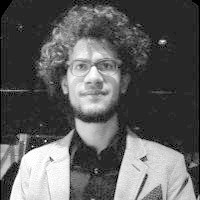
\includegraphics[width=0.15\textwidth]{photo.jpg}
		\fontsize{40pt}{60pt} % Font size
		\fontspec[Path = fonts/lato/]{Lato-Hai}\selectfont luca % First name font
		\fontspec[Path = fonts/lato/]{Lato-Lig}\selectfont rinaldi % Last name font
  	}
  	\\[5pt] % Whitespace between the name and contact information
  	\centering{ % Center the contact information
		\color{headings} % Use the headings color
		\fontspec[Path = fonts/raleway/]{Raleway-Medium}\fontsize{11pt}{14pt}\selectfont \href{mailto:asd}{asd} | 324234234234 | asdasdasd
  	} % Contact information font

	\noindent\makebox[\linewidth]{\color{headings}\rule{\paperwidth}{0.4pt}} % Horizontal rule
	\vspace{-5pt} % Reduce whitespace after the rule slightly
}


%\namesection2{Luca}{Rinaldi}{ % Your name
%\urlstyle{same}\url{https://www.linkedin.com/in/lucarin91} \\ % Your website, LinkedIn profile or other web address
%\href{mailto:lucarin91@gmail.com}{lucarin91@gmail.com} | +39 338 7845158 % Your contact information
%}
%----------------------------------------------------------------------------------------
%	LEFT COLUMN
%----------------------------------------------------------------------------------------

\begin{minipage}[t]{0.33\textwidth} % The left column takes up 33% of the text width of the page



%------------------------------------------------
% Education
%------------------------------------------------

\section{Education}
  \subsection{scuola}
  \descript{roba}
  \location{asd - asd | pisa \\ tanto}

  \sectionspace % Some whitespace after the section

%------------------------------------------------
% Coursework
%------------------------------------------------

\section{Language}

\subsection{italiano}
\location{Native}
  \subsection{inglese}
  \location{B1}
  \sectionspace % Some whitespace after the section

%------------------------------------------------
% Skills
%------------------------------------------------

\section{Skills}
  \subsection{skill}
    c \textbullet{}
\sectionspace % Some whitespace after the section

%------------------------------------------------
% Links
%------------------------------------------------

\section{Links}

LinkedIn:// \href{https://www.linkedin.com/in/lucarin91}{\bf lucarin91} \\
Github:// \href{https://github.com/lucarin91}{\bf lucarin91} \\
\sectionspace % Some whitespace after the section

%----------------------------------------------------------------------------------------

\end{minipage} % The end of the left column
%\hfill
%
%----------------------------------------------------------------------------------------
%	RIGHT COLUMN
%----------------------------------------------------------------------------------------
%
\begin{minipage}[t]{0.66\textwidth} % The right column takes up 66% of the text width of the page

%------------------------------------------------
% Experience
%------------------------------------------------

\section{Experience}

%------------------------------------------------

\runsubsection{\href{http://teamble.com/h-ack-my-vodafone}{H-ACK MY VODAFONE}}
\descript{| Developer}

\location{Marzo 2015 | Milan}
%\vspace{\topsep} % Hacky fix for awkward extra vertical space
%\begin{tightitemize}
%\item collaborazione col team di sviluppo della \textit{start-up}
%\item tesi di laurea triennale sulle tecniche di \textit{geocoding}
%\end{tightitemize}
I took 24 hours hackathon with the goal of simplifying and renewing the My Vodafone App for the Italian market. Teamwork with developers, marketers and graphic designers.

\sectionspace % Some whitespace after the section

%------------------------------------------------

\runsubsection{\href{http://pisa.coderdojo.it/}{Pisa CoderDojo}}
\descript{| co-Founder}

\location{Febrary 2015 - active | Pisa}

Together with some friends, we are organizing the CoderDojo at the SMS Biblio (Local Council Library) in Pisa. a voluntary activity to teach programming languages to the children (mostly scratch and python).

\sectionspace % Some whitespace after the section

%------------------------------------------------

\runsubsection{FreeMonkey}
\descript{| Director }

\location{July 2012 - September 2014 | Camerino(MC)}
I founded a business aiming to organise Music and Social Events in the town of Macerata. I improved my organization skills and technical competences in Audio and Lighting techniques.

\sectionspace % Some whitespace after the section

%------------------------------------------------

%------------------------------------------------
% Projects
%------------------------------------------------

\section{School Projects}

\runsubsection{\href{https://github.com/MCSN-project2014/APproject}{FunW@p}}
\descript{Programming Language}

\location{December 2014 - June 2015 }
A very simple programming language that - at the end of the work - would be compiled into F# and interpreted by a basic VM. C#, Coco/R and F# are the main tools we are using.

\sectionspace % Some whitespace after the section

%------------------------------------------------

\runsubsection{\href{https://github.com/lucarin91/mean-payoff_game}{Mean-payoff Game: Algorithms and Optimization}}
\descript{Thesis}

\location{February 2014 - September 2014 }
An application of the Game Theory to computer science. I studied the problem of mean-pay off and different algorithms to solve it. I then found some optimizations and performed experiments in C.
\sectionspace % Some whitespace after the section

%------------------------------------------------

\runsubsection{\href{https://github.com/sfcoding-school/party-manager}{Party Manager}}
\descript{Android app}

\location{March 2014 - June 2014 }
A cloud mobile app for organizing events within a group of people, through the Q&A mechanism. The cloud API is implemented using Flask and PostgreSQL.

\sectionspace % Some whitespace after the section

%------------------------------------------------

\section{Projects}

\runsubsection{\href{https://github.com/PisaCoderDojo/coderDojo-site}{PisaCOderDojo}}
\descript{Site}

\location{Febrary 2015 - active}
Pisa CoderDojo  Website. I wrote the front-end and an administration panel in Angularjs and Bootstrap, whereas for RestFull back-end I used Php with Slim Micro-Framework and Sqlite3.
\sectionspace % Some whitespace after the section

%----------------------------------------------------------------------------------------

\runsubsection{\href{https://github.com/sfcoding/webService-deployer}{webService-deployer}}
\descript{webApp deployer}

\location{March 2015}
A Perl and bash application for setting up and deploying web apps (python, nodejs, php) in a Linux+Nginx+Passenger environment, using a git server. The system automatically installs all needed library and starts the application.

\sectionspace % Some whitespace after the section

%------------------------------------------------


\end{minipage} % The end of the right column

%----------------------------------------------------------------------------------------
%	SECOND PAGE (EXAMPLE)
%----------------------------------------------------------------------------------------

%\newpage % Start a new page

%\begin{minipage}[t]{0.33\textwidth} % The left column takes up 33% of the text width of the page

%\section{Example Section}

%\end{minipage} % The end of the left column
%\hfill
%\begin{minipage}[t]{0.66\textwidth} % The right column takes up 66% of the text width of the page

%\section{Example Section 2}

%\end{minipage} % The end of the right column

%----------------------------------------------------------------------------------------

\end{document}
